% ****** Start of file apssamp.tex ******
%
%   This file is part of the APS files in the REVTeX 4.1 distribution.
%   Version 4.1r of REVTeX, August 2010
%
%   Copyright (c) 2009, 2010 The American Physical Society.
%
%   See the REVTeX 4 README file for restrictions and more information.
%
% TeX'ing this file requires that you have AMS-LaTeX 2.0 installed
% as well as the rest of the prerequisites for REVTeX 4.1
%
% See the REVTeX 4 README file
% It also requires running BibTeX. The commands are as follows:
%
%  1)  latex apssamp.tex
%  2)  bibtex apssamp
%  3)  latex apssamp.tex
%  4)  latex apssamp.tex
%
\documentclass[%
 reprint,	
%superscriptaddress,
%groupedaddress,
%unsortedaddress,
%runinaddress,
%frontmatterverbose, 
%preprint,
showpacs,
% preprintnumbers,
%nofootinbib,
%nobibnotes,
%bibnotes,
 amsmath,amssymb,
 aps,
 prc,
%prb,
%rmp,
%prstab,
%prstper,
%floatfix,
]{revtex4-1}

\usepackage{graphicx}% Include figure files
\usepackage{dcolumn}% Align table columns on decimal point
\usepackage{bm}% bold math
\usepackage{url}
\usepackage{lipsum}
\usepackage{color}
\usepackage{hyperref}% add hypertext capabilities
\usepackage[mathlines]{lineno}% Enable numbering of text and display math
\usepackage{upgreek}
\usepackage{biolinum}
% \linenumbers\relax % Commence numbering lines

%\usepackage[showframe,%Uncomment any one of the following lines to test 
%%scale=0.7, marginratio={1:1, 2:3}, ignoreall,% default settings
%%text={7in,10in},centering,
%%margin=1.5in,
%%total={6.5in,8.75in}, top=1.2in, left=0.9in, includefoot,
%%height=10in,a5paper,hmargin={3cm,0.8in},
%]{geometry}

% \setcounter{secnumdepth}{5}
\begin{document}

\preprint{APS/123-QED}

\title{Measurement of $\phi$-meson Production in Au+Au Collisions at ${\sqrt{s_{\rm NN}} = \rm{3\,GeV}}$}% Force line breaks with \\
%\thanks{A footnote to the article title}%

% \author{Ann Author}
% \altaffiliation[Also at ]{Physics Department, XYZ University.}%Lines break automatically or can be forced with \\
% \author{Second Author}%
% \email{Second.Author@institution.edu}
% \affiliation{% Authors' institution and/or address\\ This line break forced with \textbackslash\textbackslash
% }%

\collaboration{STAR Collaboration}
\noaffiliation

\date{\today}% It is always \today, today,
             %  but any date may be explicitly specified

\begin{abstract}


We report on the first measurement of $\phi$-meson production and $\phi/K^-$ ratio in Au+Au collisions at ${\sqrt{s_{\rm NN}} = \rm{3\,GeV}}$ with RHIC/STAR experiment under fixed target configuration. $\phi$-mesons are measured through their hadronic decay channel, $\phi\rightarrow K^+K^-$. The transverse momentum ($p_T$) spectra of $\phi$-mesons and $K^-$ are presented in different centrality and rapidity intervals. The total production yields and $\phi/K^-$ ratio in $4\pi$ acceptance are calculated and compared to thermal model predictions. The grand canonical ensemble (GCE) calculation shows a clear discrepancy from our measurement. Our data favors the canonical ensemble (CE) model with a strangeness correlation length $(r_c   \sim 3.2_{-0.1}^{+0.4} \rm{fm})$ in 0-10\% central Au+Au collisions at ${\sqrt{s_{\rm NN}} = \rm{3\,GeV}}$.


%\begin{description}
%\item[Usage]
%Secondary publications and information retrieval purposes.
%\item[PACS numbers]
%May be entered using the \verb+\pacs{#1}+ command.
%\item[Structure]
%You may use the \texttt{description} environment to structure your abstract; use the optional argument of the \verb+\item+ command to give the category of each item. 
%\end{description}
\end{abstract}

\pacs{25.75.-q, 25.75.Cj}% PACS, the Physics and Astronomy
                             % Classification Scheme.
%\keywords{Suggested keywords}%Use showkeys class option if keyword
                              %display desired
\maketitle

% Chapter one
% \section{Introduction}
% \label{introduction}

Relativistic heavy ion physics is aimed for detail investigation of phase structures of strongly interacting matter, governed by Quantum Chromodynamics (QCD), under extreme high temperature and density conditions. Particle production has been studied to investigate the properties of the produced QCD matter in heavy ion collisions, e.g. Equation-of-State (EoS) 


Recently measurements of $\phi$-meson over $K^-$ ratio in heavy-ion collisions show a relative enhancement in the low energies below the NN threshold compare to the high energies at RHIC and LHC. These enhancement were observed both in Au+Au collisions and also in the lighter system such as Ni+Ni, Ar+KCl and Al+Al at low energies. The grand canonical ensemble (GCE) statistical model shows a discrepancy with the measured data while the calculations from canonical ensemble (CE) with different strangeness correlation length ($r_c$) can reasonable reproduce this feature. In the GCE, the strangeness was conserved in average for the collision system, while the $r_c$ parameter in CE model corresponding to the strangeness local conserved volume size. Due to the uncertainties in the current measurements, a solid determination on the $r_c$ and distinguish those different models are still missing. The Fixed-Target program at STAR covers the center-of-mass energy (cms) from 3.0 GeV to 7.7 GeV which can map the unmeasured cms range to have a better constrain on the model calculations and understanding the strangeness production mechanisms~\cite{}.


The dataset used in this analysis consists of Au+Au collision at fixed-target (FXT) mode with ${\sqrt{s_{\rm NN}} = \rm{3\,GeV}}$ collected in the 2018 RHIC run. Approximately 2.6$\times 10^{8}$ minimum bias triggered events with 0--80\% centrality pass the selection criteria and are used in this analysis. The main detectors used are the Time Projection Chamber (TPC), the Time of Flight (TOF) detector and the Beam-Beam Counter (BBC). Events are selected with the offline reconstructed collision vertex within 1.5 cm of the target centers along the beam direction to ensure a valid collision. $\phi$ mesons are reconstructed via the hadronic decay channel $\phi\rightarrow K^+K^-$ with a branching ratio ($B.R.$) of 49.2\%~\cite{pdg}. Charged kaon tracks are reconstructed with the TPC and identified via a combination of the ionization energy loss ($dE/dx$) measurement with the TPC and the time-of-flight ($tof$) measurement with the TOF detector which have been extensively used in many prior STAR analyses. The trigger system is provide by the BBC detector. Both the TPC and TOF detectors have full azimuthal coverage with a pseudo-rapidity range of 0$<$\,$\eta$\,$<$\,2 for TPC and 0$<$\,$\eta$\,$<$\,1.5 for TOF at FXT mode~\cite{TPC,TOF}. 




Figure~\ref{fig:phiSignal} left shows the invariant mass distributions of $K^+K^-$ pairs in the $p_{T}$ region of 0.4--1.6 GeV/$c$ for 0--60\% minimum bias collisions. The combinatorial background is estimated with the mixed-event (ME) technique in which $K^+$ and $K^-$ from different events of similar characteristics (centrality, event plane angle) are paired. The mixed-event spectra are normalized to the same-event (SE) distributions in the mass range of 1.04--1.08\,GeV/$c^2$. After the subtraction of the combinatorial background from the SE kaon pairs, the remainder distributions are shown as red solid circles in the bottom. The residual $K^+K^-$ invariant mass distributions are fit to a breit-wigner plus linear function. The linear function is used to represent remaining correlated background. The $\phi$ meson raw yields are extracted from the breit-wigner function fit results and the systematic uncertainty on the extracted raw yield is evaluated using different method such as binning counting.


\begin{figure}
\centering
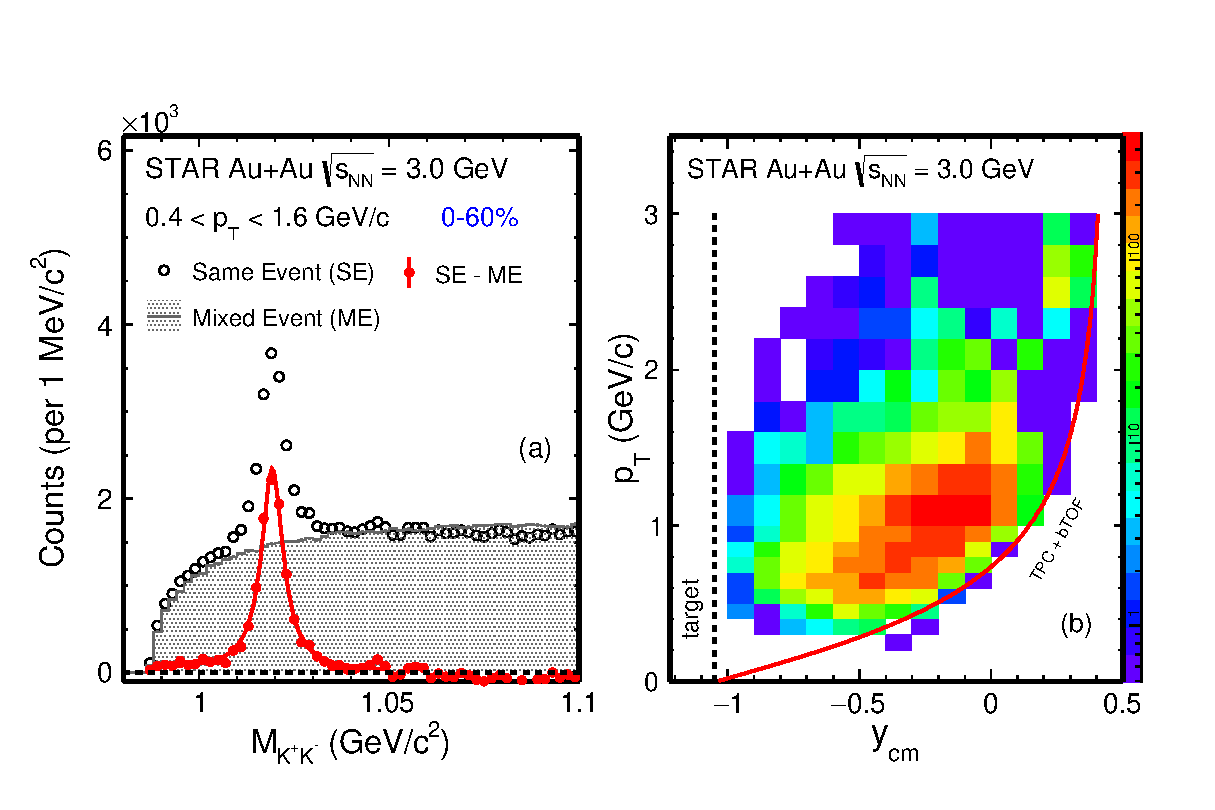
\includegraphics[width=0.50\textwidth]{fig/fig1_signal.eps}
  \caption{(a) Invariant mass of $K^+K^-$ pairs in 0-60\% centrality and 0.4--1.6\,GeV/$c$. Black open circles represent the same-event (SE) unlike-sign (US) distributions. Grey shaded histograms represent the mix-event (ME) US distributions that are used to estimate the combinatorial background. The red solid circles depict the $\phi$-meson signals obtained by subtracting the ME combinatorial background from the SE distributions. (b) The reconstructed $\phi$-meson acceptance $p_T$ vs. rapidity in the center-of-mass frame ($y_{\rm cm}$).}
\label{fig:phiSignal} 
\end{figure}


The reconstructed $\phi$ meson acceptance ($p_T$ vs. $y_{cm}$) is shown on the right panel of Fig.~\ref{fig:phiSignal}. The target is located around $y_{cm}$ = -1.05 whereas the convention use the beam-going direction as the positive direction. The red curve represent the TPC and TOF acceptance edges where the reconstructed data covers most of the mid-rapidity acceptance. 


The reconstructed $\phi$ meson and $K^-$ raw yields are calculated in each centrality and $p_{T}$ bin within each rapidity slices. The corrected $\phi$ meson and $K^-$ production invariant yields are calculated using the following formula:
\begin{equation}
  \begin{aligned}
& \frac{d^2N}{2\pi p_{T}dp_{T}dy} = \frac{1}{\rm B.R.} \times \frac{N^{\rm raw}}{N_{\rm evt} 2\pi p_{T}\Delta p_{T}\Delta y} \\
& \times \frac{1}{\varepsilon_{\rm TPC}\times\varepsilon_{\rm PID}},
  \end{aligned}
\label{equ:invariantyield}
\end{equation}
where B.R. is the corresponding decay branching ratio, $N^{\rm raw}$ is the reconstructed raw counts, $N_{\rm evt}$ is the total numbers of events in corresponding centralities. The raw yields are corrected for the TPC acceptance and tracking efficiency - $\varepsilon_{\rm TPC}$ and the particle identification efficiency - $\varepsilon_{\rm PID}$.


The uncertainty of the raw yield extraction is estimated by changing the raw yield counting method from the fit (breit-wigner function for $\phi$ meson $K^+K-$ invMass pair distribution and student-T function for $K^-$ $mass^2$ distribution) to histogram bin counting. The maximum difference between these scenarios is then converted to the standard deviation and added to the systematic uncertainties. The uncertainty of the TPC acceptance and efficiency correction $\varepsilon_{\rm TPC}$ is estimated via the standard procedure in STAR by comparing the TPC track distributions between real data and the embedding data, then by varying the track quality cuts such as the nHits fit point and dca used for tracking. After correct the corresponding efficiency for each scenarios, the difference is added to the systematic uncertainties. The uncertainty of the PID efficiency correction is estimated by varying the PID selection cuts such as the TPC $n\sigma_{K}$ and TOF $1/\eta$ and then convoluting to the final corrected yield. For the $p_T$ integrated yield measurement, limited by the acceptance, one important systematic source is from the extrapolation. We estimate this by vary several different fitting functions including levy, blast wave, $m_T$-exponential, $p_T$-exponential, $p_T$-gaussian and etc~\cite{PhysRevC.79.034909}. The maximum difference between these scenarios to the default one is then converted and quoted as the systematic source. For each individual $\phi$ meson and $K^-$ measurement, some of the uncertainties are correlated or partially correlated (eg. TPC and PID). Thus for the $\phi/K^-$ ratio measurement, in order to avoid the correlation we vary the above cuts simultaneously for $\phi$ meson and $K^-$, then quote the final ratio difference as the systematic uncertainties.


Figure~\ref{fig:phimTSpectra} shows the efficiency--corrected $\phi$ meson and $K^-$ invariant yield as a function of transverse kinetic energy ($m_T-m_0$) for various rapidity regions in 0-10\% central Au+Au collisions at ${\sqrt{s_{\rm NN}} = \rm{3\,GeV}}$. $\phi$ meson and $K^-$ spectra in some rapidity species are scaled with arbitrary factors indicated on the figure for clarity. Dashed and solid lines depict fits to the spectra with the exponential function to extrapolate the unmeasured $p_T$ ranges in order to calculate the $p_T$ integrated yield.


\begin{figure}
\centering
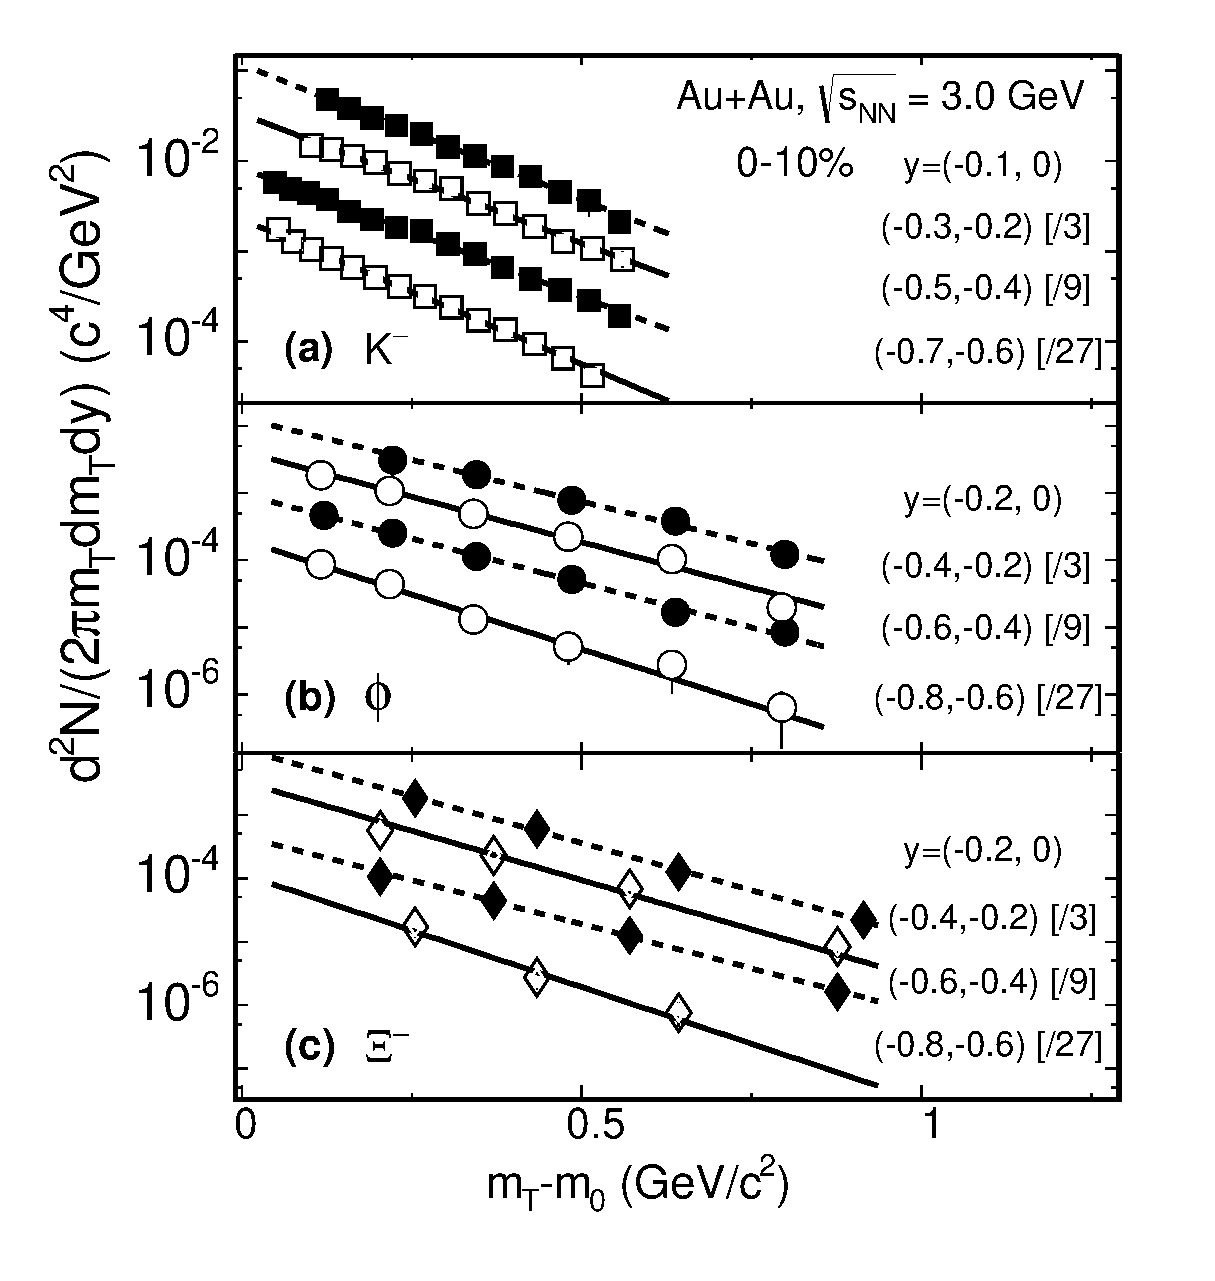
\includegraphics[width=0.41\textwidth]{fig/fig2_h_mT_spectra_phiMeson.eps}
  \caption{ $\phi$-meson and $K^-$ invariant yield as a function of transverse kinetic energy ($m_T-m_0$) for various rapidity regions in 0-10\% central Au+Au collisions at ${\sqrt{s_{\rm NN}} = \rm{3\,GeV}}$. Solid and dashed black lines depict exponential function fits to the measured data points.}
\label{fig:phimTSpectra} 
\end{figure}


Figure~\ref{fig:phiYSpectra} shows the rapidity distributions of $\phi$-meson and $K^-$ $p_T$-integrated yields $dN/dy$ in Au+Au collisions at ${\sqrt{s_{\rm NN}} = \rm{3\,GeV}}$ for three different centralities. The full symbols show the measured data, while the open ones are reflected data with respect to $y=0$ in the center-of-mass frame. Solid lines depict Gaussian function fits to the data points and used to extrapolate the unmeasured rapidity windows to calculate the $4\pi$ acceptance yields.


\begin{figure*}
\centering
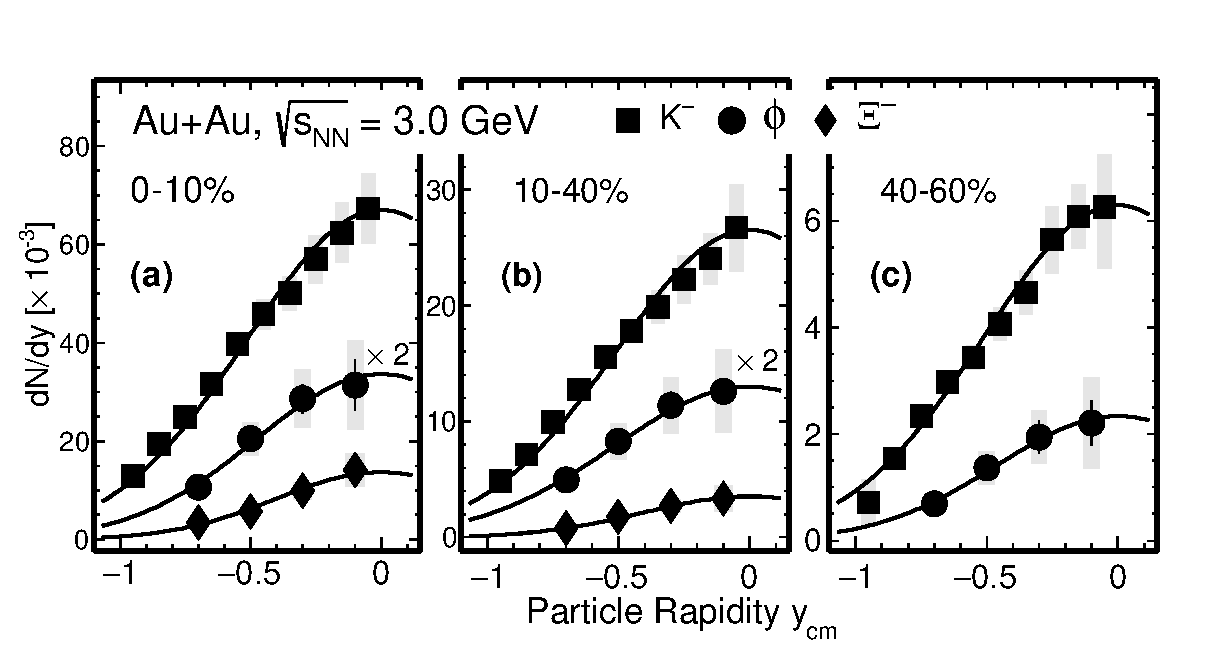
\includegraphics[width=0.8\textwidth]{fig/fig3_dndy.eps}
  \caption{ Rapidity distributions of $K^-$ (squares) and $\phi$-meson (circles) $p_T$-integrated yields $dN/dy$ in 0-10\% (a), 10-40\% (b) and 40-60\% (c) Au+Au collisions at ${\sqrt{s_{\rm NN}} = \rm{3\,GeV}}$. The full symbols show the measured data, while the open ones are reflected data with respect to $y=0$ in the center-of-mass frame. Solid lines depict Gaussian function fits to the data points.}
\label{fig:phiYSpectra} 
\end{figure*}


Figure~\ref{fig:phi2Kratio} shows the $\phi/K-$ ratio as a function of collision energy $\sqrt{s_{\rm NN}}$. The colored full symbols show these measurements in three centrality bins in Au+Au collisions at ${\sqrt{s_{\rm NN}} = \rm{3\,GeV}}$.


\begin{figure}
\centering
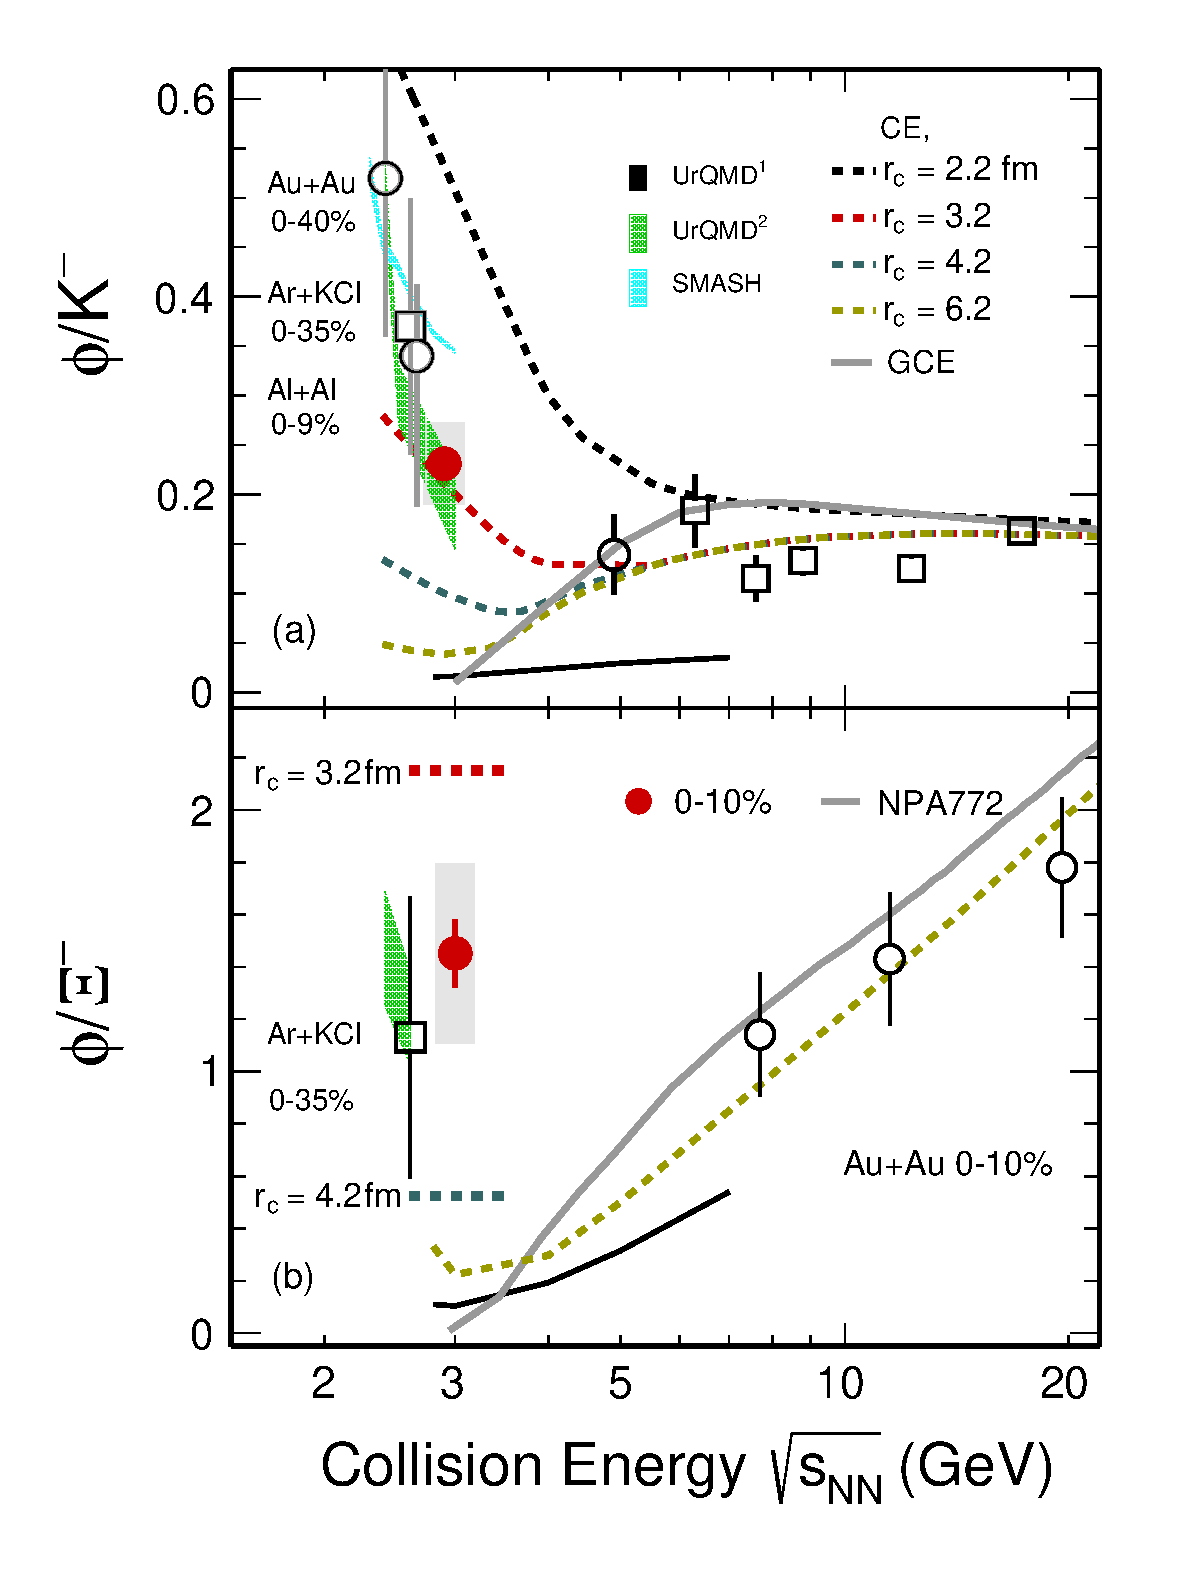
\includegraphics[width=0.41\textwidth]{fig/fig4_phi_over_kminus_zoomin.eps}
  \caption{ $\phi/K-$ ratio as a function of collision energy $\sqrt{s_{\rm NN}}$. The colored full symbols show these measurements in three centrality bins, whereas the other data points represented by different markers from various energies and collision system. The red arrow depict the $\phi$-meson production threshold in proton-proton collisions. The grey solid line represents a thermal model calculation based on grand canonical ensemble (GCE) while the dotted lines depict these calculations based on canonical ensemble (CE) with four different parameters of strangeness correlation radius ($r_c$).}
\label{fig:phi2Kratio} 
\end{figure}

Compare to models ...


In summary ...



% Chapter acknowledgement
%\section{Acknowledgement}
%\label{acknowledgement}

We thank the RHIC Operations Group and RCF at BNL, the NERSC Center at LBNL, and the Open Science Grid consortium for providing resources and support. This work is supported in part by the Office of Nuclear Physics within the U.S. DOE Office of Science, the U.S. National Science Foundation, the Ministry of Education and Science of the Russian Federation, National Natural Science Foundation of China, Chinese Academy of Science, the Ministry of Science and Technology of China and the Chinese Ministry of Education, the National Research Foundation of Korea, GA and MSMT of the Czech Republic, Department of Atomic Energy and Department of Science and Technology of the Government of India; the National Science Centre of Poland, National Research Foundation, the Ministry of Science, Education and Sports of the Republic of Croatia, RosAtom of Russia and German Bundesministerium f{\"u}r Bildung, Wissenschaft, Forschung and Technologie (BMBF) and the Helmholtz Association.

\bibliography{phi3GeV}

\end{document}
%
% ****** End of file apssamp.tex ******
